%%%%% Document Setup %%%%%%%%

\documentclass[10pt, twocolumn]{revtex4}    % Font size (10,11 or 12pt) and column number (one or two).

\usepackage{times}                          % Times New Roman font type

\usepackage[a4paper, left=1.85cm, right=1.85cm,
 top=1.85cm, bottom=1.85cm]{geometry}       % Defines paper size and margin length

\usepackage[font=small,
labelfont=bf]{caption}                      % Defines caption font size as 9pt and caption title bolded


\usepackage{graphics,graphicx,epsfig,ulem}	% Makes sure all graphics works
\usepackage{amsmath} 						% Adds mathematical features for equations

\DeclareMathOperator{\sech}{sech}		% Defining sech so it doesn't italicise it 
\DeclareMathOperator{\Int}{Int}		% Defining 'integer part of' so it doesn't italicise it 
\providecommand{\e}[1]{\ensuremath{\times 10^{#1}}} %shorthand for scientific notation

\usepackage{etoolbox}                       % Customise date to preferred format
\makeatletter
\patchcmd{\frontmatter@RRAP@format}{(}{}{}{}
\patchcmd{\frontmatter@RRAP@format}{)}{}{}{}
\renewcommand\Dated@name{}
\makeatother

\usepackage{fancyhdr}

\pagestyle{fancy}                           % Insert header
\renewcommand{\headrulewidth}{0pt}
\lhead{L. P. Flower}                          % Your name
\rhead{Collisions of Matter-Wave Solitons in a Bose-Einstein Condensate}            % Your report title               

\def\bibsection{\section*{References}}        % Position reference section correctly


%%%%% Document %%%%%
\begin{document}                     


\title{Collisions of Matter-Wave Solitons in a Bose-Einstein Condensate} 
\date{Submitted: \today{}}
\author{L. P. Flower}
\affiliation{\normalfont Durham University L3 Computing Project}

\begin{abstract}              
 
In this report we investigate the relation between amplitude and speed for solitary waves in water, given by $c = \sqrt{gh} \left(1 + \frac{\eta}{2h} \right)$. Measurements were taken visually in a 3 m wave tank, and a straight-line fit for the data was produced with $\chi_\nu^2$ = 3.3, showing a poor fit. The best-fit gradient and intercept values did not agree well with the theoretical predictions either, leading to a discussion of the experimental limitations. We also investigated the properties of soliton reflection and concluded that a phase shift is not observed in this situation, contrary to what might be expected, but that energy is lost in reflection and hence the soliton amplitude and speed decrease. 

\end{abstract}

\maketitle
\thispagestyle{plain} % produces page number for front page


%%%%%%%%%%%%%%%%%%%%%%%%%%%

\section{Introduction and Theory} \label{Intro}

In natural units and with rescaled length and time variables, the Schrodinger equation is dimensionless. Introducing an effective potential term $g |\psi|^2$ which characterises the interactions between the particles, we find the Gross-Pitaevskii equation \cite{Gross} \cite{Pitaevskii}
\begin{equation}
i \frac{\partial \psi}{\partial t} = -\frac{\partial^2 \psi}{\partial x^2} + V \psi.
\end{equation}

Define $\zeta$ as a parameter to characterise width, with units 1/length. We then have the normalised wavefunction 
\begin{equation} 
\psi(x) = \sqrt{\frac{\zeta}{2}} \sech{(\zeta x)} e^{i v x + \phi},
\end{equation}
where $v$ is the velocity of the soliton and $\phi$ is a phase factor. 
Substituting the $v=0$ case into the time-independent Schrodinger equation and setting E to be $\zeta^2$, we find $g=-4\zeta$. 

Describing the interparticle interaction by a pseudopotential approximation is valid in the dilute limit, where the average spacing between gas particles is greater than the scattering length, $a_s$. 

The rescaled length and time depend on the parameters of the experimental system which is modelled by the simulation. If a Bose-Einstein condensate of Rubidium-87 atoms has been chosen, with a scattering length of $a_s = 100 a_0$ and 5000 atoms per soliton. The radial confinement frequency $\omega_r$, which has been ignored in the computational part of this project to reduce the problem to 1D, is 800 Hz. The interaction parameter $g = 2\hbar \omega_r a_s N$ is then 4.44 \e{-34} kg m$^3$s$^{-2}$, leading to a characteristic soliton length $\tilde{x}$ which we define as the unit of rescaled length. $\tilde{x} = \frac{\hbar^2}{mg}$ where $m$ is the mass of each $^{87}$Rb atom. For this imaginary but realistic experimental setup, $\tilde{x} = $ 17.1 nm. To ensure that the Schrodinger equation is dimensionless, the unit of time must be $\tilde{t} = \frac{\hbar^3}{10mg^2}$ which evaluates to 0.856 ns.

The Gross-Pitaevskii equation was solved numerically using the split-step Fourier method for rescaled time $t$. The space-time box was initially 20x20 for the purpose of obtaining preliminary results, and was increased to 40x40 for repeated collisions. Initially 2000, then 4000 space points and 4000 time points were used to minimise discretization effects. In order for this simulation to accurately represent an experiment, it must be run over a time period of at least a few milliseconds, corresponding to $\tilde{t}$ from 0 to 200,000. For the simulation to complete in a reasonable time, $\delta t \approx 100$ since the model is $O(1)$ complexity [is it?]. However, this would lead to inconsistencies in the model due to the presence of a harmonic confining potential in the case of repeated collisions, where a smaller timestep improves the integrability of the soliton solutions. A compromise has been reached in this model where $\delta t$ is small, but the extent of time is not comparable to real experiments in most cases. 

%%%%%%%%%%%%%%%%%%%%%%%%%%%%%%%%%%%%%%%%%%%%%%%%%%%%%%%

\section{Methods} \label{Methods}

The split-step Fourier method is a mathematical trick borrowed from optics and relies on the fact that in Fourier space, the operator $\frac{d}{dx}$ becomes $k$, the transformed variable with units 1/length. Once the wavefunction has been propagated in k-space, the inverse Fourier transform is taken. The potential energy term is approximated as a product of two half-exponentials (this is inexact as the potential depends on $|\psi|^2$) which are incorporated in the wavefunction propagation. The wavefunction at a time $t+\delta t$ is then given by

\begin{equation} \label{fft}
\psi(x,t+\delta t) = e^{-\frac{i(V+g|\psi|^2 \delta t}{2}} \mathcal{F}^{-1}[e^{i(2\pi k)^2 \delta t} \mathcal{F} [e^{- \frac{i(V+g|\psi|^2) \delta t}{2}} \psi(x,t) ] ],
\end{equation}
where $V$, $g$ and $\psi$ are defined above in the Gross-Pitaevskii equation. 

The discrete $k$ values are found from $\delta k = \frac{1}{n \delta x}$. The Fast Fourier Transform module \texttt{numpy.fft} was used to compute the discrete Fourier tranforms and inverses. 

%%%%%%%%%%%%%%%%%%%%%%%%%%%%%%%%%%%%%%%%%%%%%%%%%%%%%%%

\section{Preliminary Results} \label{Milestone}

 For $\zeta=1$, it was found by trial and error that $g=-4$ confined the soliton, in perfect agreement with theory. The norm $|\psi|^2$ was integrated over the interval $(-2,2)$, giving a probability leakage of 0.012\% over the extent of the experiment, $\tilde{t}$ from 0 to 20. 

\begin{figure}[h]
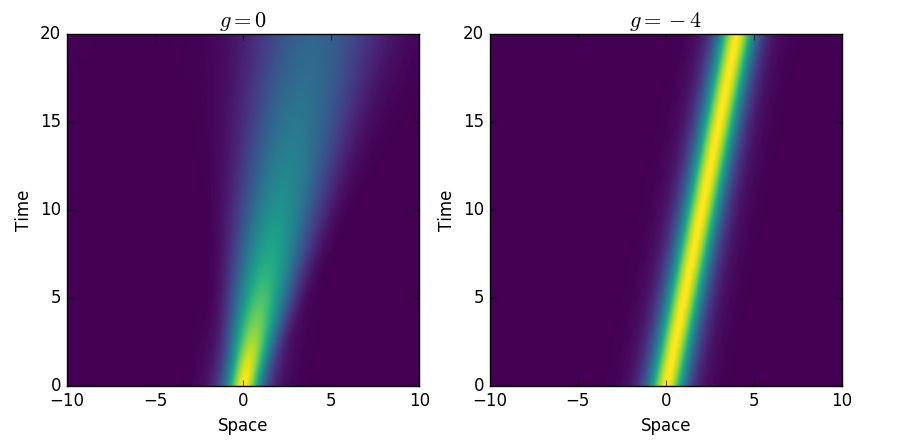
\includegraphics[width=\columnwidth]{milestonepic.png}
\captionof{figure}{A graph showing the effect of inter-atom interactions $g |\psi|^2$ on a soliton model. The family 
parameter $\zeta = 1$ hence $g=-4$ perfectly confines the soliton with velocity $v=0.2$.}
\end{figure}

%%%%%%%%%%%%%%%%%%%%%%%%%%%



To investigate the properties of solitary waves, we filled a wave tank with water and used a sluice to create solitons. The tank was 30 cm deep, 15.2 cm wide and 2.98 m long. We used a water depth of 8 cm, since to use the predictions of the KdV equation (see Section \ref{Intro}), the soliton amplitude must be significantly less than that of the water, but we found with a larger volume of water in the tank the waves were likely to spill over. We filled the sluice with water at depths between 10.5 cm and 14.5 cm to produce at least one visible soliton which endured long enough to take measurements. Rapidly removing the sluice gate leaves a rectangular disturbance in the tank, which evolves eventually into one or more solitons with different amplitudes and hence different speeds. 

\begin{figure}[h]
%\includegraphics[width=\columnwidth]{diagram1-NoReflections.png}
\caption{The experimental setup for measuring the speed of solitons with no reflections involved.}
\label{Diagram1}
\end{figure}

As you can see in Fig. \ref{Diagram1}, a camera was set up near the equipment so as to be able to see both vertical rulers, which formed the start and end points of the velocity measurement and were 1.5 m apart. From this distance it was not possible to see the dark metal rulers, so we marked the tank to compare with the wave amplitude. After the sluice gate was removed, the camera began recording and each frame was associated with the time it was taken. The first few seconds of frames were not analysed, as the solitons had not completely evolved and their shape was still changing. The photos which showed a fully formed primary soliton travelling between the two rulers were analysed and the mean soliton speed over that distance calculated.

Soliton amplitude gradually decreases as a result of energy lost in collisions with the tank walls, so we repeated the measurement at later times on the same soliton. As its amplitude decreased, its speed decreased and so we assumed these were valid measurements, equivalent to producing new solitons using a smaller volume of water in the sluice. By repeating this process with differing volumes of water in the sluice, we obtained repeats for most soliton amplitudes (measured to the nearest 0.25 cm) and took the weighted mean of the velocites.

\begin{figure}[h]
%\includegraphics[width=\columnwidth]{diagram2-Reflections.png}
\caption{The setup for observing the reflections of solitons off the wave tank wall.}
\label{Diagram2}
\end{figure}

As shown in Fig. \ref{Diagram2}, to measure properties of solitons undergoing collisions with the tank wall, we again used a vertically placed ruler both to measure amplitude and to provide a reference point for measuring distances, and hence speed. The distance between the left-hand edge of the ruler and the wall of the wave tank was 0.49 m. The method for taking measurements was very similar to the case with no reflection: the time between the soliton passing the ruler travelling to the left, and then travelling to the right, was found using the photos taken by the camera, and hence the speed calculated. Our hypothesis was that a soliton would 'pause' on reflection, described mathematically as acquiring a phase shift, before travelling back at the same speed. Testing this was complicated by the fact that the soliton amplitude often decreased after the reflection as a result of lost energy (since the water viscosity is obviously non-zero). In this case, theoretically the soliton should emerge from the collision travelling at a slower speed. By using the speed data as measured without reflections, we can evaluate the importance of each effect. If we compare the expected time elapsed, had the collision with the tank wall only affected the soliton's amplitude, with the actual time elapsed as measured by the camera, we can evaluate whether the phase shift hypothesis is correct. 

%%%%%%%%%%%%%%%%%%%%%%%%%%%

\section{Results} \label{Results}

\subsection{Collisions}

\subsection{Repeated Collisions}

\begin{figure}[h]
%\includegraphics[width=\columnwidth]{noReflections-residuals.png}
\caption{The green points with error bars show the measured velocity of solitons plotted against their measured amplitude, and the black line shows the best fit to these points. The orange area shows the theoretical velocity prediction for that amplitude, with the associated error. The normalised residuals of the data to the fit are plotted below.}
\label{Graph1}
\end{figure}

We begin by considering the velocity measurements taken over a single length of the wave tank. The data were plotted in Fig. \ref{Graph1}, and a straight-line fit obtained using weighted least squares. The best-fit gradient, $a$, was 3.2 $\pm$ 0.3 s$^{-1}$, the best-fit intercept, $b$, was 0.913 $\pm$ 0.004 m s$^{-1}$ and the minimised $\chi^2$ value was 22.8. As there were nine data points and two fit parameters, $\nu$ = 7 and hence the reduced chi-squared $\chi_\nu^2$ was found to be 3.3. 


Next, we look at the second experimental setup, involving solitons approaching the wave tank wall, reflecting off it and travelling away again, sometimes with significantly reduced amplitude and speed. We know from previous research and the KdV equation that solitons undergoing overtaking collisions emerge unscathed except for a slightly reduced amplitude and a phase shift, advancing the faster wave and retarding the slower \cite{Segur}. We aimed to investigate whether a similar mechanism applies to a soliton reflecting off a wall, in effect colliding head-on with itself. 

\begin{figure}[h]
%\includegraphics[width=\columnwidth]{reflections-residuals.png}
\caption{The green points show the measured speed of solitons, including the reflection, plotted against their initial measured amplitude. The orange area, as before, shows the theoretical velocity prediction for that amplitude with its error.}
\label{Graph2}
\end{figure}

After repeat readings were collated it became clear that one data point was anomalous: its measured velocity was more than 10\% larger than the theoretical velocity for the measured amplitude. Also, the error in speed was $\approx$10\%, compared to errors of 2-4\% for every other data point. This point was therefore omitted from Fig. \ref{Graph2} and from the gradient, intercept and $\chi^2$ calculations. 

A weighted least-squares fit was used to find the best-fit gradient, $a$ = 4.1 $\pm$ 0.1 s$^{-1}$ and the intercept, $b$ = 0.856 $\pm$ 0.002 m s$^{-1}$. With these values of $a$ and $b$, $\chi^2_{min}$ = 1.8. There were seven data points, so $\chi_\nu^2$ = 0.37. For a good fit we would expect  $\chi_\nu^2 \approx$ 1, so in this case the errors in velocity have been overestimated. Looking at the graph, we can see that all the data points are fairly near the line of best fit, but their errors are large, so all points are within one standard error bar of the best fit line (rather than two-thirds of the points as would be expected). It may have been beneficial to obtain repeated observations of the same wave, to reduce the error on the time measurement. However, this would only work if the observations agreed, otherwise combining them does not improve the overall result. This is not guaranteed as there is evidence for subjectivity in the visual method of measuring time differences.

Despite the low chi-squared value, the strong straight-line fit with speed values lower than those predicted suggests that the reflection has a definite effect on the soliton, even though it does not destroy it nor even change its shape. The possible effects we have considered are a decrease in amplitude resulting in a lower speed and an imparted phase shift delaying the soliton’s return. 

To try to quantify the effect of reflection on a soliton's speed, we can look back at the non-reflecting speed data. As well as calculating the speed of solitons travelling across the tank, the method of data collection meant that we could measure the time taken for the wave to reflect off the tank wall between measurements. We can also calculate the time we would expect this to take, if indeed the reflection is like that of waves on a string at open boundaries: distance to the tank wall divided by speed travelling to the left, plus distance back again divided by speed travelling to the right. By observing the difference between these times, we can conclude whether reflection imparts a phase shift, and hence a retarding time shift, on solitons. 

Table \ref{Table} below shows the results of inferring the time shift which occurred in the solitons produced as they reflected off the wave tank wall. In the table, $t_0$ is the expected time elapsed between passing a reference point before and after the reflection, if only soliton speed was affected; $t_m$ is the actual (measured) time elapsed and $t_m - t_0$ is the difference between them - the time shift. 

\begin{figure}[h!]
\begin{tabular}{| c | c | c |} % three centre-justified columns
\hline
$t_0$ /s & $t_m$ /s & $t_m - t_0$ /s $\pm$ 0.04 s \\ \hline
4.599	& 4.761 		& 0.162 \\ \hline
4.538	& 4.599 		& 0.061 \\ \hline
4.717	& 4.679		& -0.038 \\ \hline
4.481	& 4.520		& 0.039 \\ \hline
4.539	& 4.561		& 0.022 \\ \hline
4.720	& 4.602		& -0.118 \\ \hline
4.386	& 4.459		& 0.073 \\ \hline
4.601	& 4.562		& -0.039 \\
\hline
\end{tabular}
\caption{A table showing time shifts in solitons after reflection off a tank wall. The error in each time difference is 0.04 s.}
\label{Table}
\end{figure}

%%%%%%%%%%%%%%%%%%%%%%%%%%%

\section{Discussion} 

The gradient obtained for speed-amplitude data as plotted in Fig. \ref{Graph1} was 3.2 $\pm$ 0.3 s$^{-1}$, which is lower than the theoretical gradient of $\sqrt{g/4h} =$ 5.54 $\pm$ 0.03 s$^{-1}$. They differ by more than 3 standard error bars, which indicates disagreement with theory \cite{Hughes}. In this section we will consider reasons for the disagreement including suitability of the equipment, experimental practice and analysis techniques. 

The intercept was found to be 0.913 $\pm$ 0.004 m s$^{-1}$, slightly higher than the theoretical value of 0.886 $\pm$ 0.006 m s$^{-1}$. The values differ by less than 3 standard errors, so there is clearly some agreement. The weak agreement could be a result of a too-low gradient, as the speeds were approximately correct compared to the theoretical predictions at the amplitude values considered. For lower amplitude solitons, which we could not accurately describe here because they were hard to see, lower speeds might be observed which could correct the gradient. Also, the intercept could easily be influenced by mistakes in amplitude measurement, so we calculated the amplitude underestimation which would completely account for the too-high intercept here as around 0.7 cm. This is much larger than the precision in amplitude, so mistakes cannot completely account for the difference. 

As stated in section \ref{Results}, the reduced chi-squared $\chi_\nu^2$ = 3.3 for this dataset. As this is greater than 3, we say that the straight-line model is a poor fit for the data. Furthermore, calculating the P-value gives $P$ = 0.002 $\approx 10^{-3}$. In this case the hypothesis that the speed-amplitude data fits a straight line must be questioned, but not rejected outright. However, there is no apparent structure in the residuals except that more points are above the line of best fit than below it. There is no obvious correction to the model here, but it seems that the two points with small velocity error lying below the theoretical prediction have had their error underestimated. This analysis suggests that the model is fundamentally correct but that the experiment described in this report had too many sources of unaccounted error, both systematic and statistical, to demonstrate the model properly.

The errors on the data points are far from equal, as some values of amplitude had only one set of data whereas others had three or four. This was due to using the same solitons at different points in their lifetimes rather than systematically repeating measurements. For certain amplitudes all repeats yielded similar speed values, whereas others differed greatly, and it would have been beneficial to collect more data on these if we had had time. Imaging and analysing these situations in detail might have revealed situations in which the model of solitary waves is not valid, such as when many background ripples are present in the tank. However, it is also possible that the measurement becomes more imprecise as soliton amplitude increases since larger solitons lose energy faster, meaning a constant uncertainty in amplitude measurement is not appropriate. 

Disturbances in the wave tank are hard to correct for - including situations where the primary soliton, which is being observed, reflects off the tank wall and immediately collides with the secondary soliton which travels more slowly. It is as yet unclear what happens to the speed of a soliton during a head-on collision because their amplitudes momentarily increase, but since solitons colliding head-on are not described by a single KdV equation, the linear relationship between velocity and amplitude may not hold. Factors such as these could explain why the speed-amplitude graph had a lower gradient than expected and did not precisely follow a straight-line fit. 

A large problem we faced when visually analysing data, particularly with reference to time measurements, was subjectivity. Whilst looking at photos together the experimentalists nearly always agreed on the time at which a soliton passed a reference point, but when analysis was done separately, and the results compared, there were often disagreements larger than the estimated error. Additionally, any outsiders looking at the same camera frames were likely to come to different conclusions. We can see especial evidence of subjectivity and bias when looking at Fig. \ref{Graph2}. The almost-constant offset of the data from the theoretical prediction points to a systematic overestimation of the time taken, which could have been amplified by the fact that in this setup (see Fig. \ref{Diagram2}) the same reference point was used twice. Additionally, we did not ensure that the camera was pointed exactly orthogonally to the direction of wave travel, neglecting the effect of decreased depth perception when looking at a photo. The effect appears to be less in Fig. \ref{Graph1} because two separate reference points were used, meaning that a bias in a particular direction was likely to be cancelled out by the same bias in the second measurement. 

The time shift values in the table in section \ref{Results} are not all positive, suggesting the possibility that the observed time shifts are in fact a random distribution centred on zero. We can test this using a hypothesis test: the null hypothesis is that the time shifts are normally distributed with a mean of zero. We take the mean of our sample of 8 measurements, $\overline{\rm \Delta t}$ = 0.0199 s and find the probability of a mean value at least as extreme as this being found by chance. We find $P(\overline{\rm \Delta t} \geq $ 0.0199$) =$ 0.409 by normalising to the standard normal distribution, using the sample standard deviation. This is only an approximate test as the distribution standard deviation would ideally be known, and the sample standard deviation found from it by dividing by the square root of the number of measurements. Even if this is only approximately correct, a P-value of 0.409 is sufficiently high that there is no evidence to support rejecting the null hypothesis. Hence, we cannot infer from this data that the mean phase shift imparted during soliton reflection is anything other than zero. 

We can conclude from this investigation that a reflection off a tank wall does not affect a soliton in the same way as undergoing an overtaking collision, and a phase shift is not observed. We can then ask why we see such low apparent velocities when a reflection is present (see Fig. \ref{Graph2}). One explanation is subjectivity, as described above. However, we must also consider that the solitons lose energy in collision and that this reduces their amplitude and, if they continue to obey the speed-amplitude relation, their speed. We have plotted the initial soliton amplitude, so perhaps a less extreme deviation from theory would be observed had we taken the average of the initial and final values. 

%%%%%%%%%%%%%%%%%%%%%%%%%%%

\section{Conclusions}
 
In conclusion, a more precise setup would be required to accurately study the properties of solitons in a wave tank. The errors associated with multiple waves being produced and interacting with each other are mostly unaccounted for here, because the methods of data collection were too subjective and the precision was too low to correct for these errors. However, we can say that reflecting off a tank wall does not impart a large phase shift onto a soliton, as might be expected if the process was similar to overtaking waves. 

If given more time to investigate solitons in water, we would use a longer wave tank (at least 6 m) with a pebble slope to absorb waves before they reflect and interact with following solitons, as described by Bettini et al. \cite{UGlab}. To study collisions between solitons we would need two sluices in the wave tank, as producing multiple solitons using a paddle did not yield useful results. A computer simulation of soliton reflection and collision may allow us to make better predictions about the outcome and find the best way to verify these experimentally. Finally, a pair of electrodes to be immersed in water would greatly improve the precision of amplitude measurement and allow us to study solitons of smaller amplitude, where the KdV equation has higher validity. 

%%%%%%%%%%%%%%%%%%%%%%%%%%%

\begin{thebibliography}{}

\bibitem{Gross} E. P. Gross (1961), "Structure of a quantised vortex in boson systems", \textit{Il Nuovo Cimento}, \textbf{20}(3) pp. 454-477. 
\bibitem{Pitaevskii}  L. P. Pitaevskii (1961), "Vortex lines in an imperfect Bose gas", \textit{Sov. Phys. JETP.} \textbf{13}(2) pp. 451–454.
\bibitem{Bound} N.-C. Panoiu, I. V. Mel’nikov, D. Mihalache, C. Etrich and F. Lederer (1999), "Multiwavelength pulse transmission in an optical fibre - Amplifier system", \textit{Phys. Rev.} \textbf{60}(4868).
\bibitem{Adams} A. D. Martin, C. S. Adams and S. A. Gardiner (2008), "Bright Solitary-Matter-Wave Collisions in a Harmonic Trap: Regimes of Soliton-like Behaviour", \textit{Physical Review A} \textbf{77}(1). 

\end{thebibliography} 

%%%%%%%%%%%%%%%%%%%%%%%%%%%

\section{Appendix: Error Analysis} \label{Errors}

In the preliminary investigation into the number of solitons which evolved from an initial rectangular disturbance, the Int function means that an error on the number of solitons cannot be found in the usual sense. Instead, we used the functional approach \cite{Hughes} to calculate the error in $S$ from the errors in $\ell$, $a$ and $h$ (which were all estimated as 1 mm). We then calculated the number of solitons which would emerge for the minimum and maximum possible values of $S$ within its error, giving a minimum and maximum number of solitons which were expected to emerge. In seven out of eight cases the minimum, predicted and maximum numbers were the same. 

The error on the depth of water was taken to be 1 mm, the smallest division on the ruler it was measured with. The error on the wave height was estimated as 2.5 mm. The resolution of the camera was limited so we could only read ruler divisions 5 mm apart, but visual estimation allowed us to distinguish between wave heights which differed by half a division. The error in the amplitude was then found by adding in quadrature the errors in depth and overall wave height. 

When visually analysing the photos of the wave tank we used the camera's measurement of the time to see when the wave crest crossed a reference point. If two photos were roughly equally close to this moment, the error on the time was taken as half the difference in these two times. If not, the error was taken as a quarter of the difference between the photo immediately after the crossing moment and the photo before (to avoid any directional bias). The error in the time difference was then found by the sum in quadrature of the errors in each time measurement. 

The error in the distance travelled by the wave was taken to be only 1 mm, as we measured this carefully multiple times. Any uncertainty in the position of the wave relative to the reference points is encapsulated in the time error rather than the distance. The error in wave velocity follows simply from these: using the multiplication/division formula \cite{Hughes}, $\alpha_v = v \sqrt{(\alpha_x/x)^2 + (\alpha_t/t)^2}$. 

We calculated the theoretical soliton velocity from the measured amplitude using equation \ref{SpeedEqn}, and evaluated the error using the functional approach, adding the contributions from errors in depth and amplitude (since both appear directly in the equation) in quadrature \cite{Hughes}. In a similar way, we evaluated the errors on the theoretical gradient, $\sqrt{g/4h}$ and intercept, $\sqrt{gh}$ using the functional approach to propagate the error in depth. 

The error on the gradient and intercept of each speed-amplitude graph was found from the minimised $\chi^2$ fit. Contours of $\chi^2$ were plotted in 2-dimensional parameter space and the error on the parameters taken to be the distance from the solution to the extrema of the $\chi^2+1$ contour. 

To estimate the error on the measured time shifts as set out in table \ref{Table}, we simply took the recording time of the camera and divided by the total number of frames, which gives the average error in a time measurement, then multiplied by $\sqrt{2}$ to obtain the error in a time difference. 

\end{document}